%!!!!!!!!!!!!!!!!!!!!!!!!!!!!!!!!!!!!!!!!!!!!!!!!!!!!!!!!!!!!!!!!!!!!!!!!!!!!!!
%!NOTE: This example file has been prepared according to the University of
%!      Hawaii Style & Policy Manual for Theses and Dissertations dated
%!      "Revised September 2010". If you have one with a later date, you may
%!      need to make revisions to this document as well. In any event, making
%!      sure your thesis complies with Graduate Education guidelines is
%!      ultimately your responsibility. Caveat LaTeXtor. :)
%!!!!!!!!!!!!!!!!!!!!!!!!!!!!!!!!!!!!!!!!!!!!!!!!!!!!!!!!!!!!!!!!!!!!!!!!!!!!!!

%% The options are (you can only choose one from each group):
%%
%% 10pt, 11pt, 12pt: chooses the point size for the document. "11pt" is the
%%                   default.
%%
%% oneside, twoside: whether you want your document onesided or twosided. Note
%%                   that twosided is not guaranteed to work, and style
%%                   guidelines prohibit double sided printouts on final
%%                   copy. "oneside" is the default.
%%
%% draft, final: when printing drafts you can save a lot of paper by using the
%%               "draft" option. It switches to single spacing, displays overful
%%               hboxes with a black box, prints a version number on title page 
%%               and omits signature page. Of course for the final copy make
%%               sure to use the "final" option! "final" is the default.
%%
%% thesis, dissertation: switches between the style for a master's thesis and a 
%%                       Ph.D. dissertation. The differences are fairly minor
%%                       and limited to the front matter. "thesis" is the
%%                       default.
%%
%% actual, proposal: switches between actual document and proposal mode. In
%%                   proposal mode: the title page is simplified and the
%%                   version number is always printed.
%%
%%% Load the new uhthesis document class
\documentclass[12pt]{article}

\usepackage[table,xcdraw]{xcolor}
\usepackage{setspace}
\usepackage{paralist}
%\usepackage{amsmath}
\usepackage{bm}
%\usepackage{subfigure}
\usepackage{cite}
\usepackage{multirow}
\usepackage{todonotes}
\usepackage{umoline}
\usepackage{xspace}
\usepackage{soul}
%\usepackage{gensymb}
\usepackage[euler]{textgreek}
\usepackage{array}
\usepackage{tabu}
\usepackage{tabularx}
\usepackage{subcaption}
\usepackage{amsmath}
%\usepackage{table}
%\usepackage{xcolor}
%\usepackage{xcdraw}

%%% Custom Macros %%%
\newcommand\tab[1][1cm]{\hspace*{#1}}
\newcommand{\LL}[2][inline]{\todo[color=red!50,#1]{\sf \textbf{LL:} #2}\xspace}
\newcommand{\HC}[2][inline]{\todo[color=blue!50,#1]{\sf \textbf{HC:} #2}\xspace}
\newcommand{\gridsize}{\texttt{GRID\_SIZE\xspace}}
\newcommand{\celsius}{$^\circ$C\xspace}
\newcommand{\hotspot}{Hotspot\xspace}
\newcommand{\crosstalk}{crosstalk\xspace}
\newcommand{\Crosstalk}{Crosstalk\xspace}
%\newcommand{\alpha}{\textalpha }
%%% Load some useful packages:
%% New LaTeX2e graphics support
\usepackage{graphicx}
%% Package to linebreak URLs in a sane manner.
\usepackage{url}
\usepackage{float}
\usepackage{paralist}
\usepackage{listings}
\lstset{frame=tb,
  language=Python,
  aboveskip=3mm,
  belowskip=3mm,
  showstringspaces=false,
  columns=flexible,
  basicstyle={\small\ttfamily},
  numbers=left,
  numberstyle=\tiny\color{black},
  keywordstyle=\color{blue},
  commentstyle=\color{dkgreen},
  stringstyle=\color{red},
  breaklines=true,
  breakatwhitespace=true,
  tabsize=3
}
\usepackage{geometry} % Required for adjusting page dimensions and margins

\geometry{
        paper=a4paper, % Paper size, change to letterpaper for US letter size
        top=2.5cm, % Top margin
        bottom=3cm, % Bottom margin
        left=2.5cm, % Left margin
        right=2.5cm, % Right margin
        headheight=10pt, % Header height
        footskip=1.5cm, % Space from the bottom margin to the baseline of the footer
        headsep=1.2cm, % Space from the top margin to the baseline of the header
        %showframe, % Uncomment to show how the type block is set on the page
}

\usepackage{lmodern}%get scalable font
%\usepackage{showframe}
\usepackage{titling}
\pretitle{\begin{center}\fontsize{18bp}{14bp}\selectfont}
\posttitle{\par\end{center}}
\preauthor{\begin{center}\fontsize{14bp}{14bp}\selectfont}
\postauthor{\par\end{center}\vspace{14bp}}
\predate{}
\date{}
\postdate{}
\title{ICS674 Mini Project}

\author{Lambert Leong}


\begin{document}

%\textbf{ICS674 Mini Project}
%\\    Lambert Leong

\maketitle

For my evolutionary computation mini project I implemented a genetic algorithm
that matches an input string.  Code implementations are written in Python2.7.

\section{Search Space}

The search space consists of all alphabet characters, upper and lower case.
This can be seen in Listing~\ref{lst:search_space} where we randomly fill the
search strings with letters by calling \texttt{string.letters} from Pythons
string module.

\begin{lstlisting}[caption = {Search space is all letter characters, upper and
lower case }, label = {lst:search_space}]
self.string = ''.join(random.choice(string.letters) for _ in xrange(length))
\end{lstlisting}

\section{Variation Operator}

Two variation operator are implemented which include crossover and mutation.

\subsection{Crossover}

To perform crossover we we randomly select two parent strings from the previous
generation, seen in lines 4\&5 of Listing~\ref{lst:cross}.  I randomly select an
integer which corresponds to the array index at which the parent string is split
for each child to inherit, seen i line 8.  Child 1 gets the char from the first
half from parent 1 and the second half from parent 2.  Child 2 gets the first
half from parent 2 and second half from parent 1.

\begin{lstlisting}[caption = {Crossover Function}, label = {lst:cross}]
def crossover(individuals):
        offspring = []
        for _ in xrange((population - len(individuals))/2):
                parent1 = random.choice(individuals)
                parent2 = random.choice(individuals)
                child1 = Individual(in_str_len)
                child2 = Individual(in_str_len)
                split = random.randint(0, in_str_len)
                child1.string = parent1.string[0:split] + parent2.string[split:in_str_len]
                child2.string = parent2.string[0:split] + parent1.string[split:in_str_len]
                offspring.append(child1)
                offspring.append(child2)
        individuals.extend(offspring)
        return individuals
\end{lstlisting}

\subsection{Mutation}

Mutation occurs in the for of switching out a character in a search string with
a random letter.  All strings in the population are susceptible to mutation and
multiple mutation can occur in a individual string.  The mutation rate is 5\% as
indicated in line 4 of Listing~\ref{lst:mutation}.

\begin{lstlisting}[caption = {Mutation Function}, label={lst:mutation}]
def mutation(individuals):
        for individual in individuals:
                for i, param in enumerate(individual.string):
                        if random.uniform(0.0, 1.0) <= 0.05:
                                individual.string = individual.string[0:i] + random.choice(string.letters) + individual.string[i+1:in_str_len]
        return individuals
\end{lstlisting}


\section{Selection Operator}

Individual strings are sorted based upon their fitness scores, as seen in
Listing~\ref{lst:selection}.  Only the top 20\% of the individual strings are
kept for each generation, which can be seen in line 6.  Lines 3-5 are for
graphing purposes and not part of the selection function.

\begin{lstlisting}[caption = {Selection Function}, label = {lst:selection}]
def selection(individuals):
        individuals = sorted(individuals, key=lambda individual: individual.fitness, reverse=True)
        max_fit.append(max(individuals, key=lambda individual: individual.fitness).fitness)
        min_fit.append(min(individuals, key=lambda individual: individual.fitness).fitness)
        avg_fit.append(float(sum(i.fitness for i in individuals)//len(individuals)))
        individuals = individuals[:int(0.2*len(individuals))]
        return individuals
\end{lstlisting}

\section{Termination Criterion}

Listing~\ref{lst:term} displays the termination code.  The algorithm terminates
when it has reached the last generation, seen i line 1, or when the fitness is
100, seen in line 7.  Fitness scores are out of a 100 and a score of 100 equates
to an identical and successful string match.

\begin{lstlisting}[caption={Termination}, label={lst:term}]
 for generation in xrange(generations):
                generation_list.append(generation)
                individuals = fitness(individuals)
                individuals = selection(individuals)
                individuals = crossover(individuals)
                individuals = mutation(individuals)
                if any(individual.fitness >= 100 for individual in individuals):
                        found = True
                        break
\end{lstlisting}

\section{Objective Fuction}

Figure~\ref{fig:fitness} indicates the max, min, and average fitness scores in
each generation.  During this run, the string was matched in a little over 350
generation.  The blue line reaches a fitness score of 100 which is the max
fitness score and indicates a successful match of the input string which was
``HelloWorld".  Fitness scores were calculated with the objective function shown
in Listing~\ref{lst:fit}

\begin{figure}[H]
        \centering
        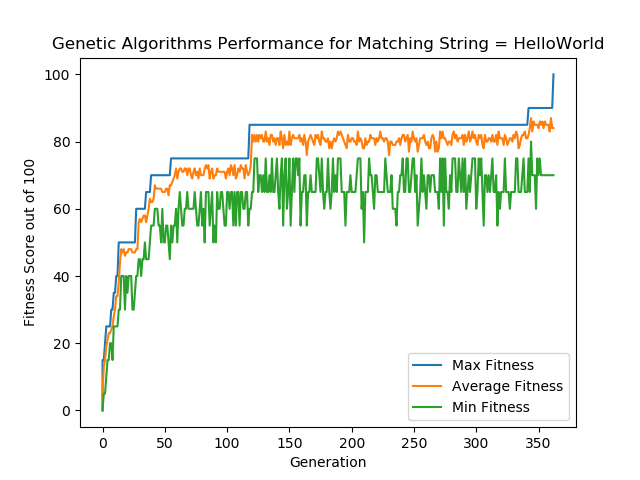
\includegraphics[width=.8\textwidth]{figures/Figure_3.png}
        \caption{Max, average, and min fitness values of each individual string
for each generation}
        \label{fig:fitness}
\end{figure}

As mentioned above, fitness scores are out of 100 and they are calculated as
percentages.  The \texttt{total} is given the value of twice the length of the
string, seen in line 3.  If the search/individual string contains a letter that
is also contained in the input string, the fitness \texttt{score} is incremented
by 1.  This process occurs in lines 9-14.  Once a letter from the search string
is found to be in the input string, that letter is removed from the input string
for future searches as to avoid duplicates and unwanted fitness score
increases.  
\\ \\
Scores are also incremented if the
search string contains the right letter in the right location or at the same
index as the input string, which can be seen in lines 5-7. The score is then
divided by the total and multiplied by 100 to get the resulting fitness score,
shown in line 15.

\begin{minipage}{\textwidth}

\begin{lstlisting}[caption = {Fitness Function}, label = {lst:fit}]
def fitness(individuals):
        for individual in individuals:
                total = len(in_str)*2
                score = 0
                for i, letter in enumerate(individual.string):
                                if in_str[i] == letter:
                                        score += 1
                compare_str = in_str
                for a_char in individual.string:
                        for i, in_char in enumerate(compare_str):
                                if a_char == in_char:
                                        score += 1
                                        compare_str = compare_str[:i]+compare_str[i+1:]
                                        break
                individual.fitness = int((float(score)/float(total))*100)                          
        return individuals
\end{lstlisting}
\end{minipage}
\end{document}
